\documentclass[12pt]{article}
\usepackage[a4paper, total={6in, 9in}]{geometry}
\usepackage{graphicx}
\graphicspath{ {./images/output/} }
\usepackage{caption}
\usepackage[english]{babel}
\usepackage{titling}
\usepackage{float}
\usepackage{amsmath}
\usepackage{minted}
\usepackage{multicol}
\usepackage{array}
\usepackage{setspace}
\usepackage{placeins}

% \usepackage{lipsum}

\title{Experiment 1\\
\textbf{Study on Industrial Robotic Trainer Kit With Different Functionality; Pick and Place Operation}}
\author{}
\date{}

\pagenumbering{gobble}
\begin{document}
\vspace*{\fill}
\begin{center}

    \emph{Heaven's Light is Our Guide} \\
    \textbf{Rajshahi University of Engineering and Technology} \\

    \begin{figure}[H]
        \centering
        
\includegraphics[scale=.34]{images/RUET_logo.png}
        \label{fig:ruet_logo}
    \end{figure}
    \vspace{5mm}

    \textbf{Course Code}\\
    MTE 4118\\
    \vspace{3mm}
    \textbf{Course Title}\\
    Control System and Robotics Sessional

    \vspace{5mm}
    \textbf{Experiment Date:} {July 8, 2025},\\
    \textbf{Submission Date:} {July 22, 2025}\\

    \vspace{5mm}
    \textbf{Lab Report 1: \\
        Study on Industrial Robotic Trainer Kit With Different Functionality; Pick and Place Operation}

    \vspace{15mm}

    \begin{tabular}{c|c}
        \textbf{Submitted to}   & \textbf{Submitted by} \\
        Md. Faisal Rahman Badal & Md. Tajim An Noor     \\
        Assistant Professor     & Roll: 2010025         \\
        Dept of MTE, RUET       &                       \\
    \end{tabular}

\end{center}
\vspace*{\fill}


\pagebreak

\tableofcontents

\pagebreak
\pagenumbering{arabic}
\maketitle

\section*{Objectives}
\addcontentsline{toc}{section}{Objectives}
\begin{enumerate}
    \item To learn about the industrial robotic trainer kit.
    \item To understand the basic operation and functionality of the industrial robotic trainer kit, with a focus on pick and place operation.
    \item To explore the application of the robotic trainer kit in performing specific industrial tasks.
\end{enumerate}

\section*{Theory}
\addcontentsline{toc}{section}{Theory}
Industrial Robotic Trainer Kits provide hands-on experience in robotics and automation, allowing students to learn programming, kinematics, and control of robotic arms in a practical setting. These kits are widely used in engineering education to teach the fundamentals of industrial automation and robotic systems \cite{groover2007automation, craig2005introduction}. They help bridge theoretical concepts with real-world applications, preparing users for careers in modern manufacturing and automation \cite{siciliano2016springer}.

\subsection*{Components}
\addcontentsline{toc}{subsection}{Components}

\subsubsection*{Trainer Kit}
\addcontentsline{toc}{subsubsection}{Trainer Kit}
The trainer kit consists of essential components for simulating industrial robotics:
\begin{enumerate}
    \item \textbf{Manipulator (ROBOTEK II)}: A multi-joint robotic arm for pick-and-place and material handling.
    \item \textbf{Hole Sensor}: Detects holes for alignment and positioning.
    \item \textbf{Part Sensor}: Identifies parts on the conveyor for accurate placement.
    \item \textbf{Conveyor Belt}: Moves items between stations, simulating industrial workflows.
    \item \textbf{Robot Control Software}: Provides programming and control via a graphical interface.
\end{enumerate}

\begin{figure}[H]
    \centering
    \begin{minipage}{0.48\textwidth}
        \centering
        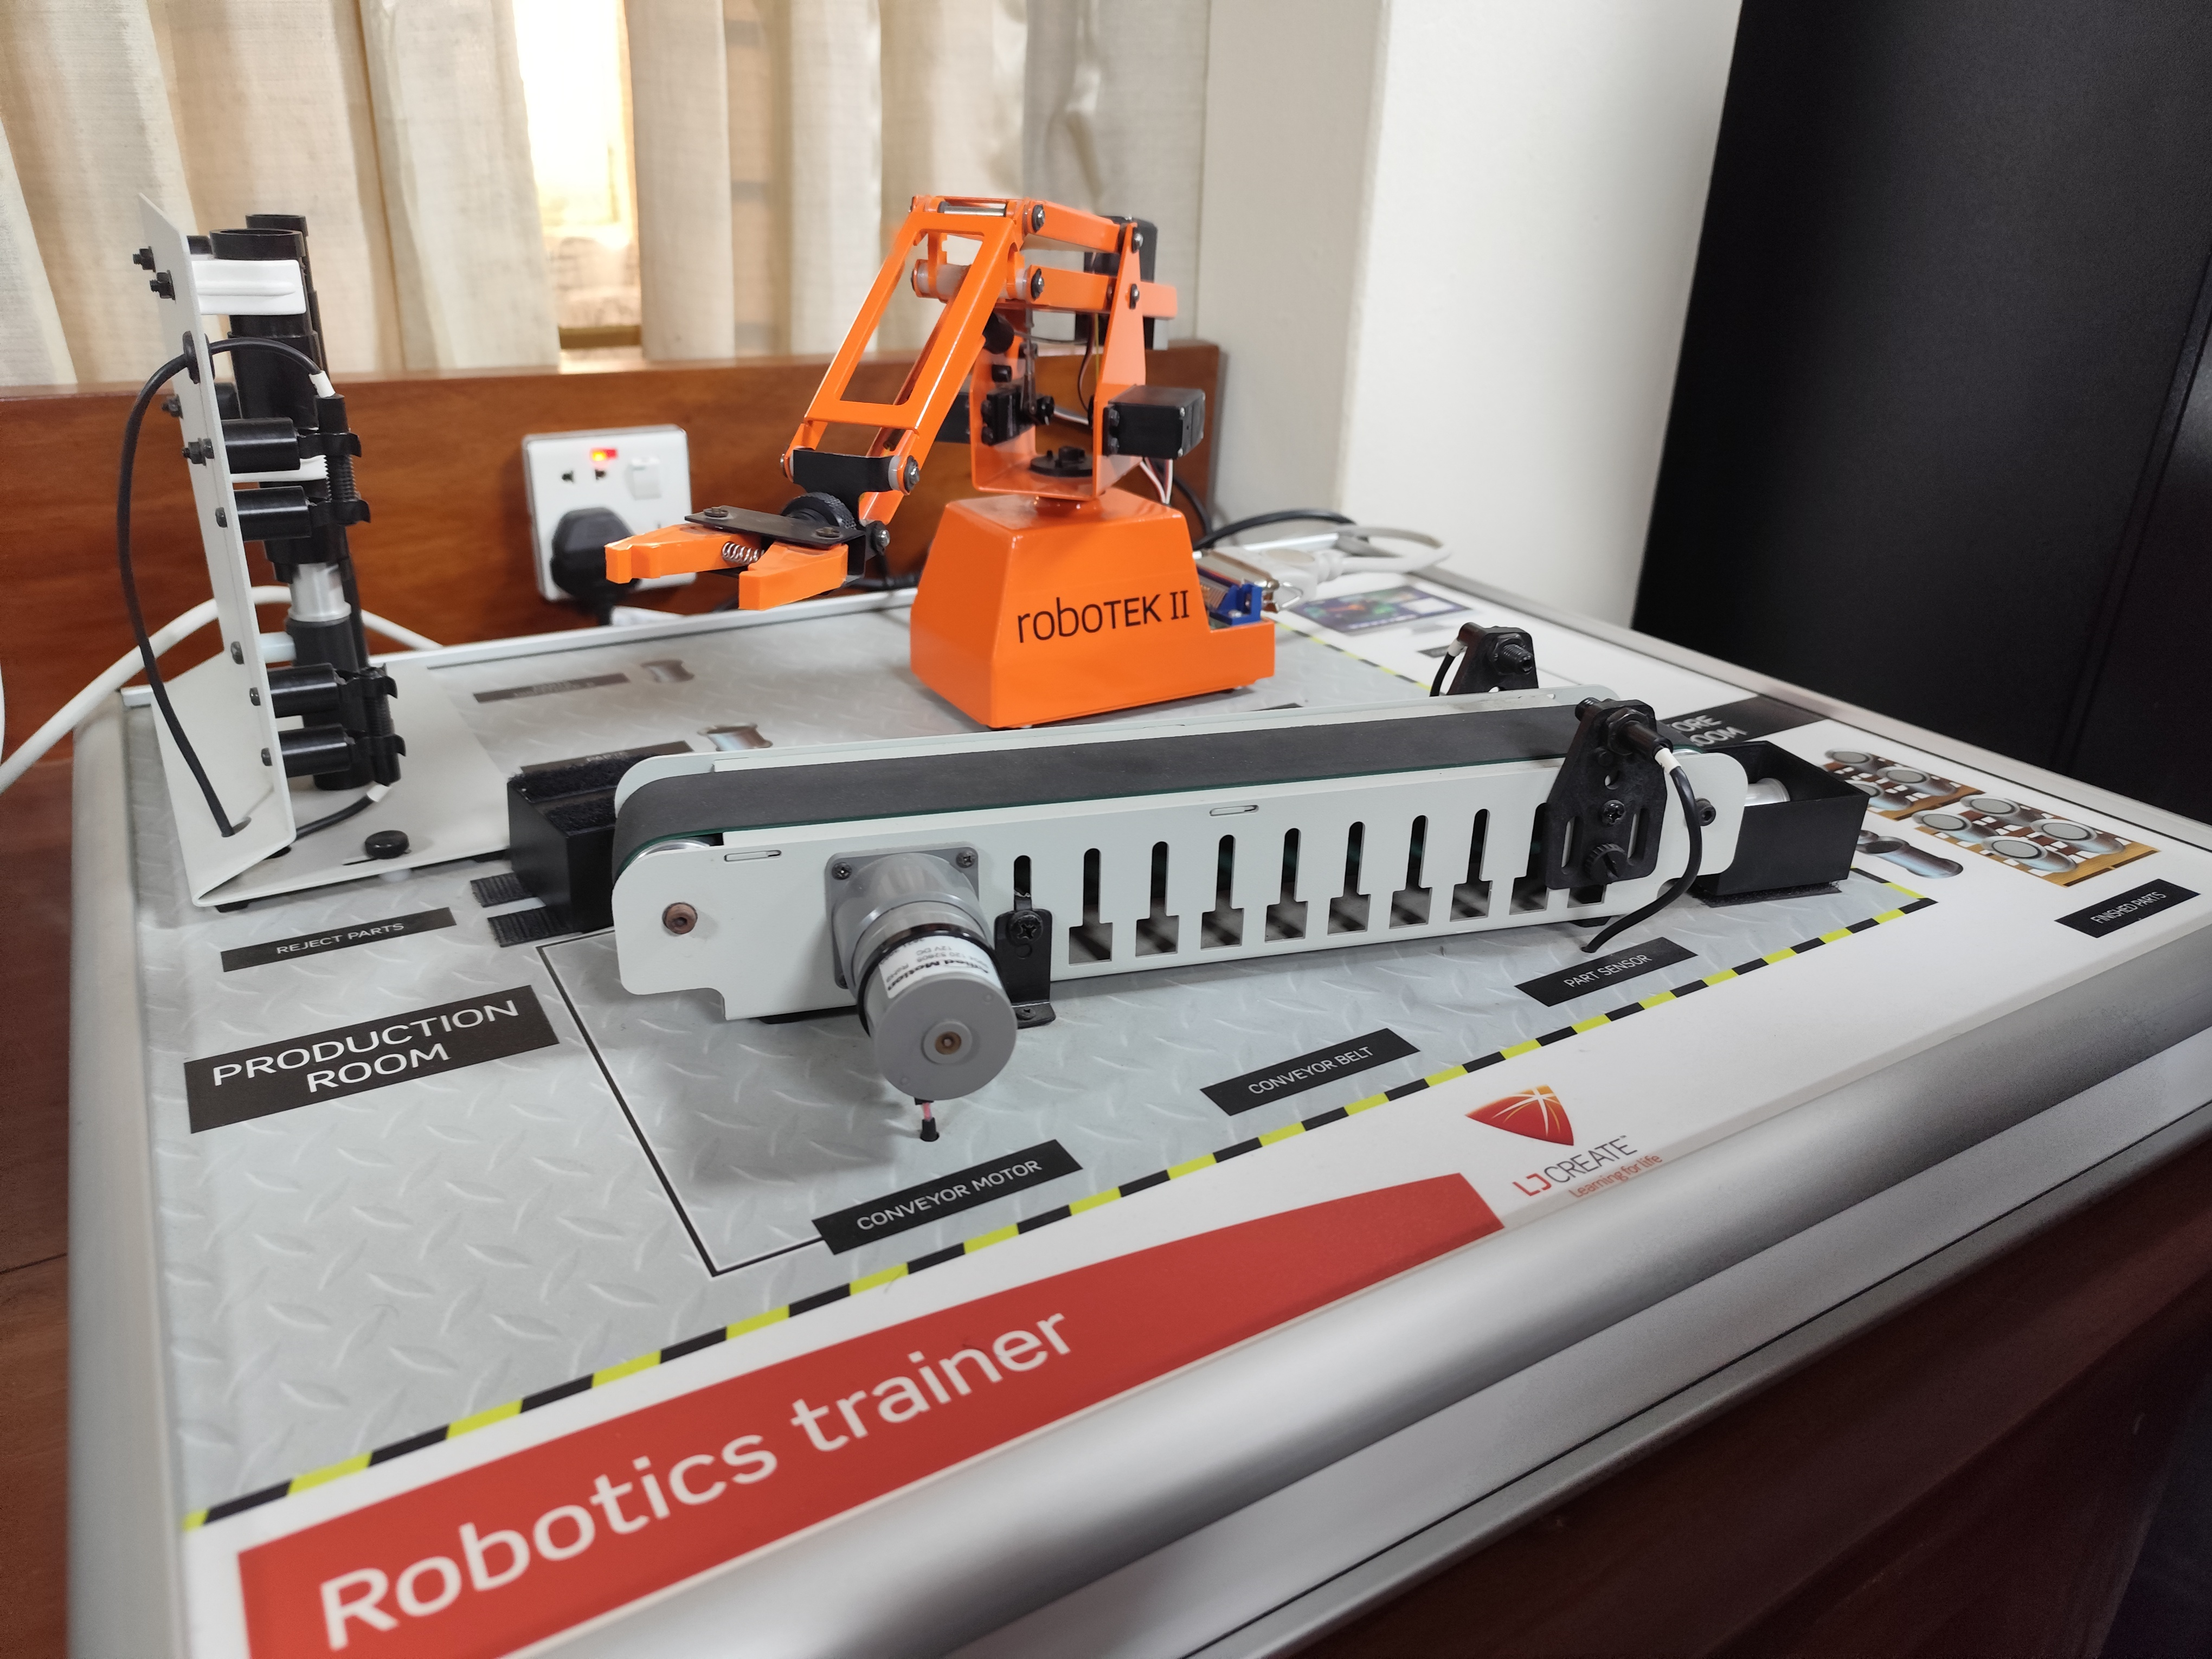
\includegraphics[width=\textwidth]{1.jpg}
        % \label{fig:trainer-kit-a}
    \end{minipage}\hfill
    \begin{minipage}{0.48\textwidth}
        \centering
        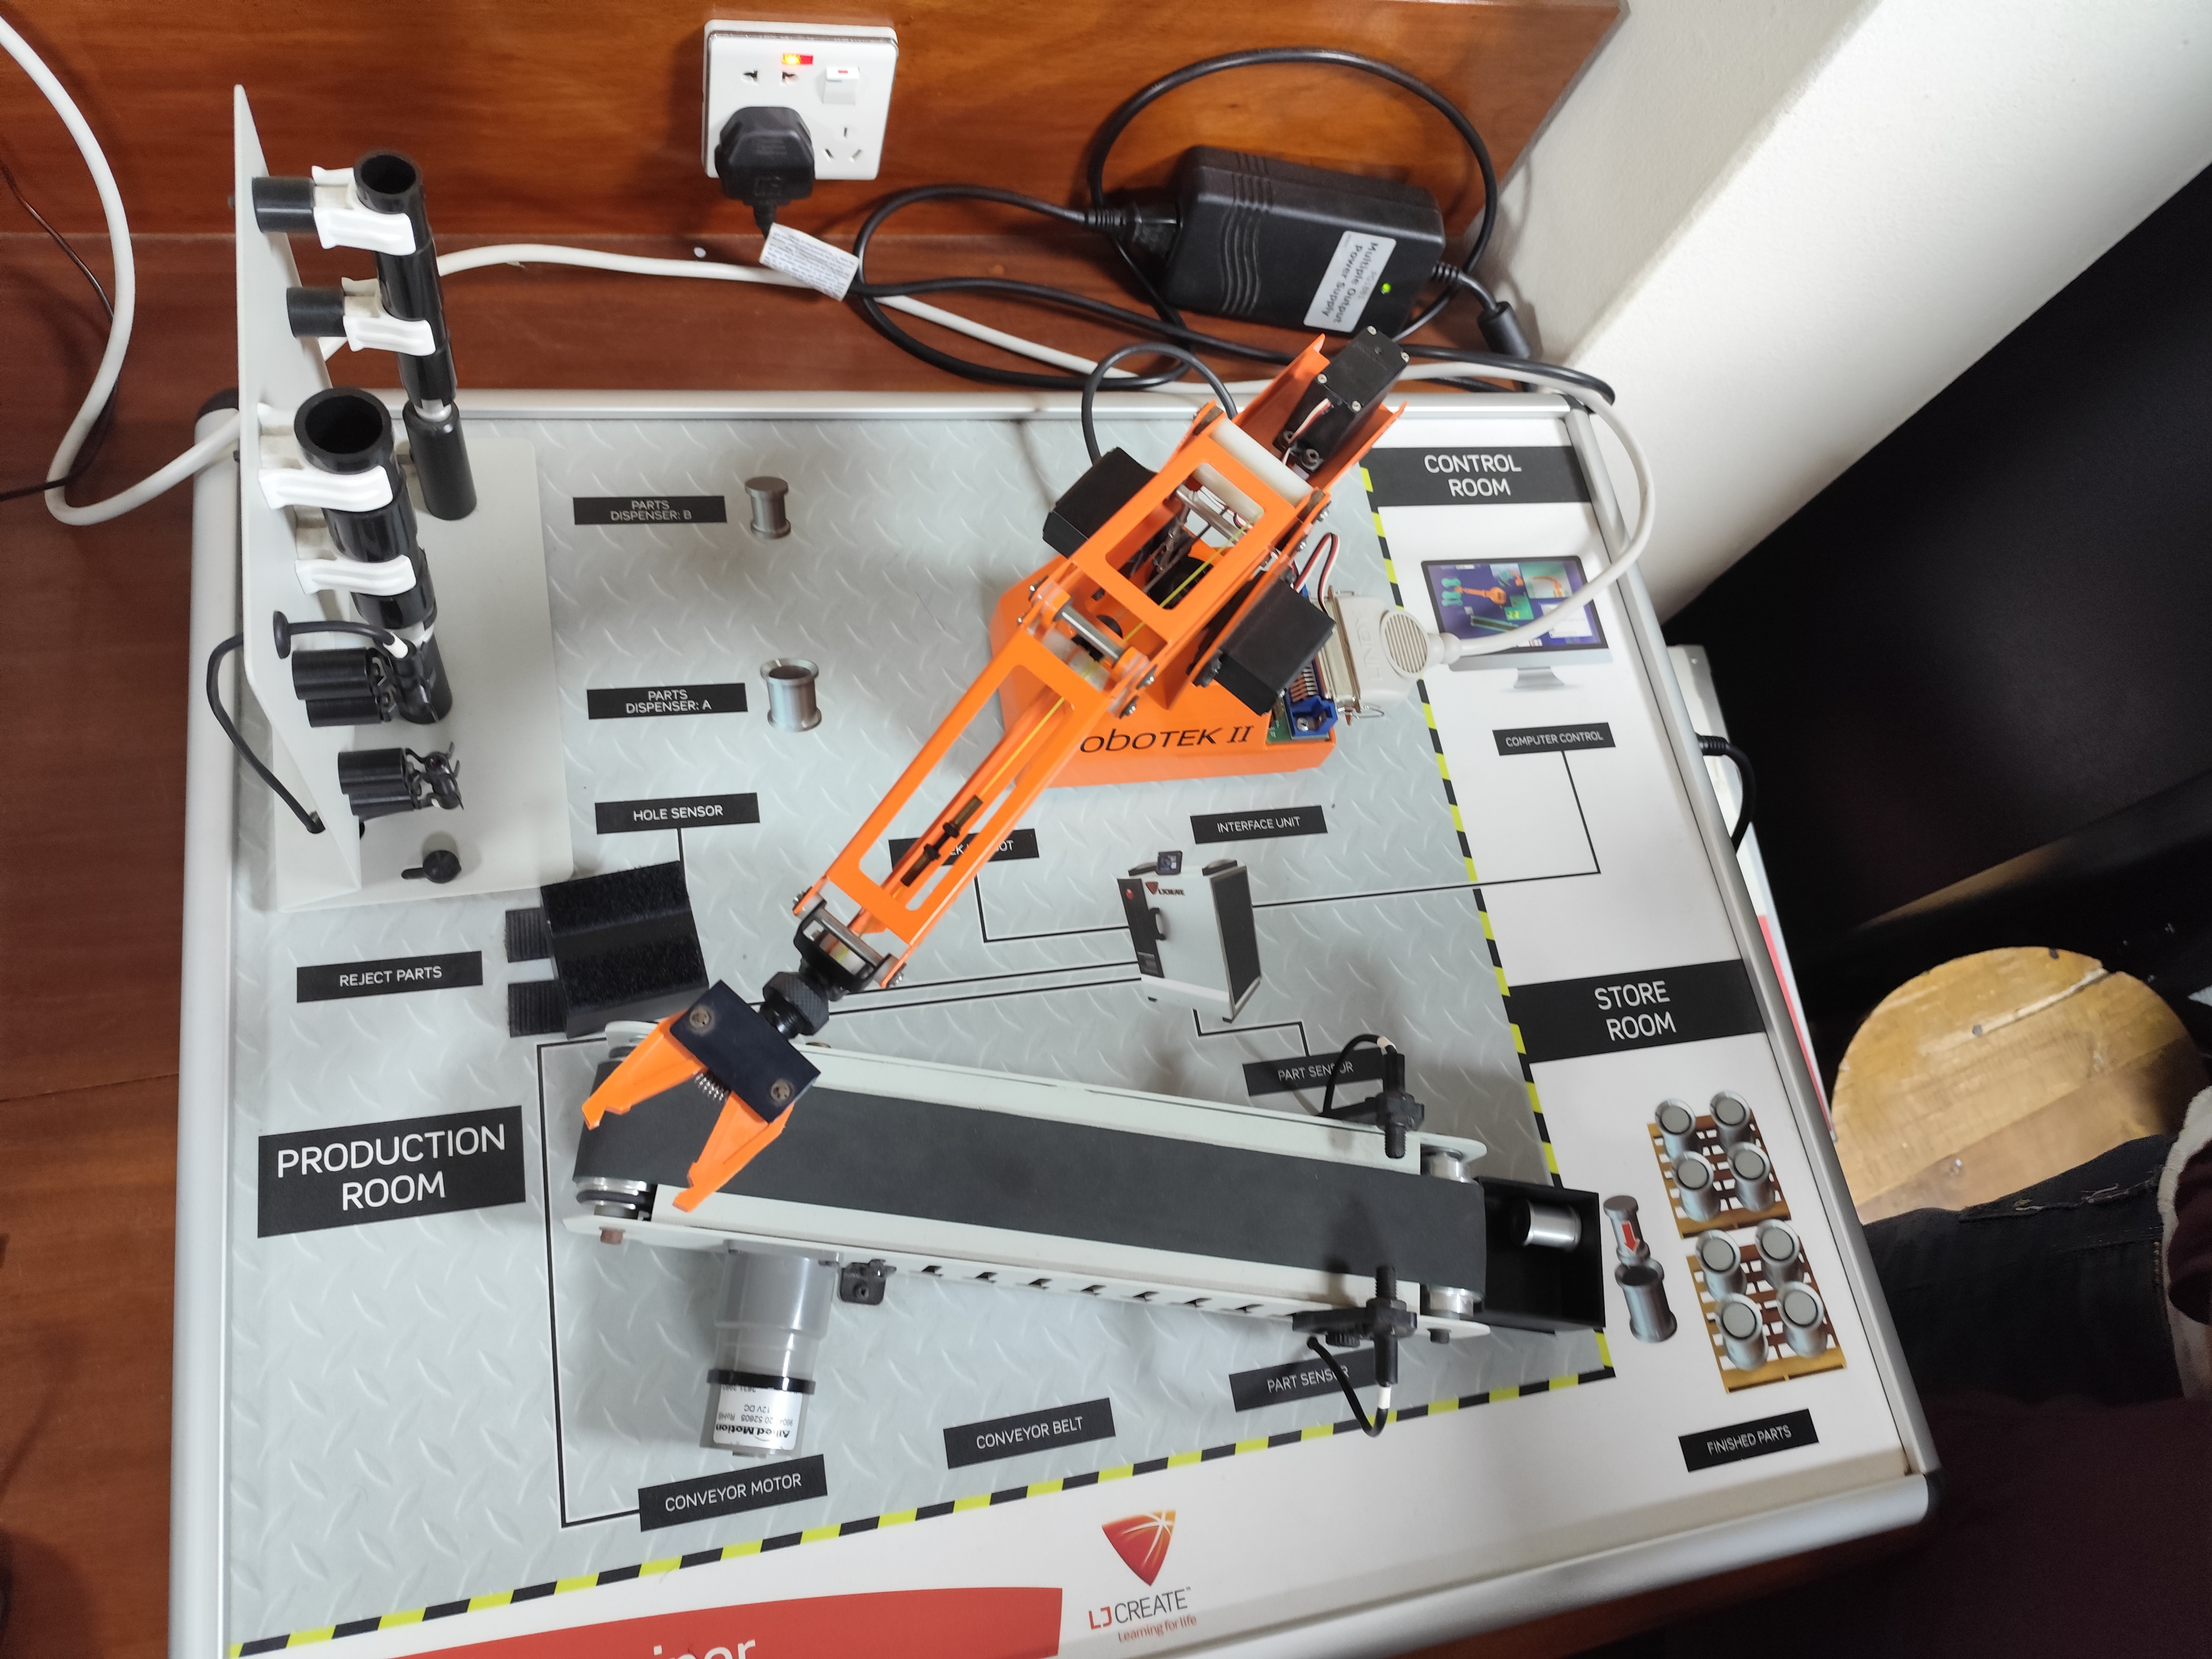
\includegraphics[width=\textwidth]{12.jpg}
        % \label{fig:trainer-kit-b}
    \end{minipage}
    \caption{Trainer Kit}
    % \label{fig:trainer-kit}
\end{figure}

\subsubsection*{Manipulator}
\addcontentsline{toc}{subsubsection}{Manipulator}
The manipulator consists of key components:

\begin{enumerate}
    \item \textbf{Power Supply}: Provides electrical energy for operation.
    \item \textbf{Shoulder}: Connects the base to the arm, enabling movement.
    \item \textbf{Arm}: Extends from the shoulder for positioning.
    \item \textbf{Jaw}: Acts as the gripper for handling objects.
    \item \textbf{Base}: Supports and stabilizes the manipulator.
\end{enumerate}

\subsubsection*{Robot Control Software}
\addcontentsline{toc}{subsubsection}{Robot Control Software}
The Robotek II manipulator uses dedicated control software with a user-friendly graphical interface. This software enables users to create, edit, and run programs, supports trajectory planning, end-effector control, and sensor integration, and provides real-time monitoring and feedback. Key features include:

\begin{enumerate}
    \item \textbf{Menu}: Access to functions and settings.
    \item \textbf{Robot Joints}: Displays and controls joint positions.
    \item \textbf{Program Editor}: For creating and managing robot programs.
    \item \textbf{Simulation}: Virtual testing of robot movements.
    \item \textbf{Sensor Integration}: Real-time sensor monitoring.
    \item \textbf{Manual Control}: Direct manipulation for setup.
    \item \textbf{Status Monitoring}: System feedback and error reporting.
    \item \textbf{Conveyors and Sensors}: Integration for automation.
    \item \textbf{Robot Control Window}: Centralized operation interface.
    \item \textbf{Actuator Window}: Adjusts actuator movements.
    \item \textbf{Sensor Window}: Displays and configures sensors.
    \item \textbf{Control Program Window}: Executes robot programs.
\end{enumerate}

\begin{figure}[H]
    \centering
    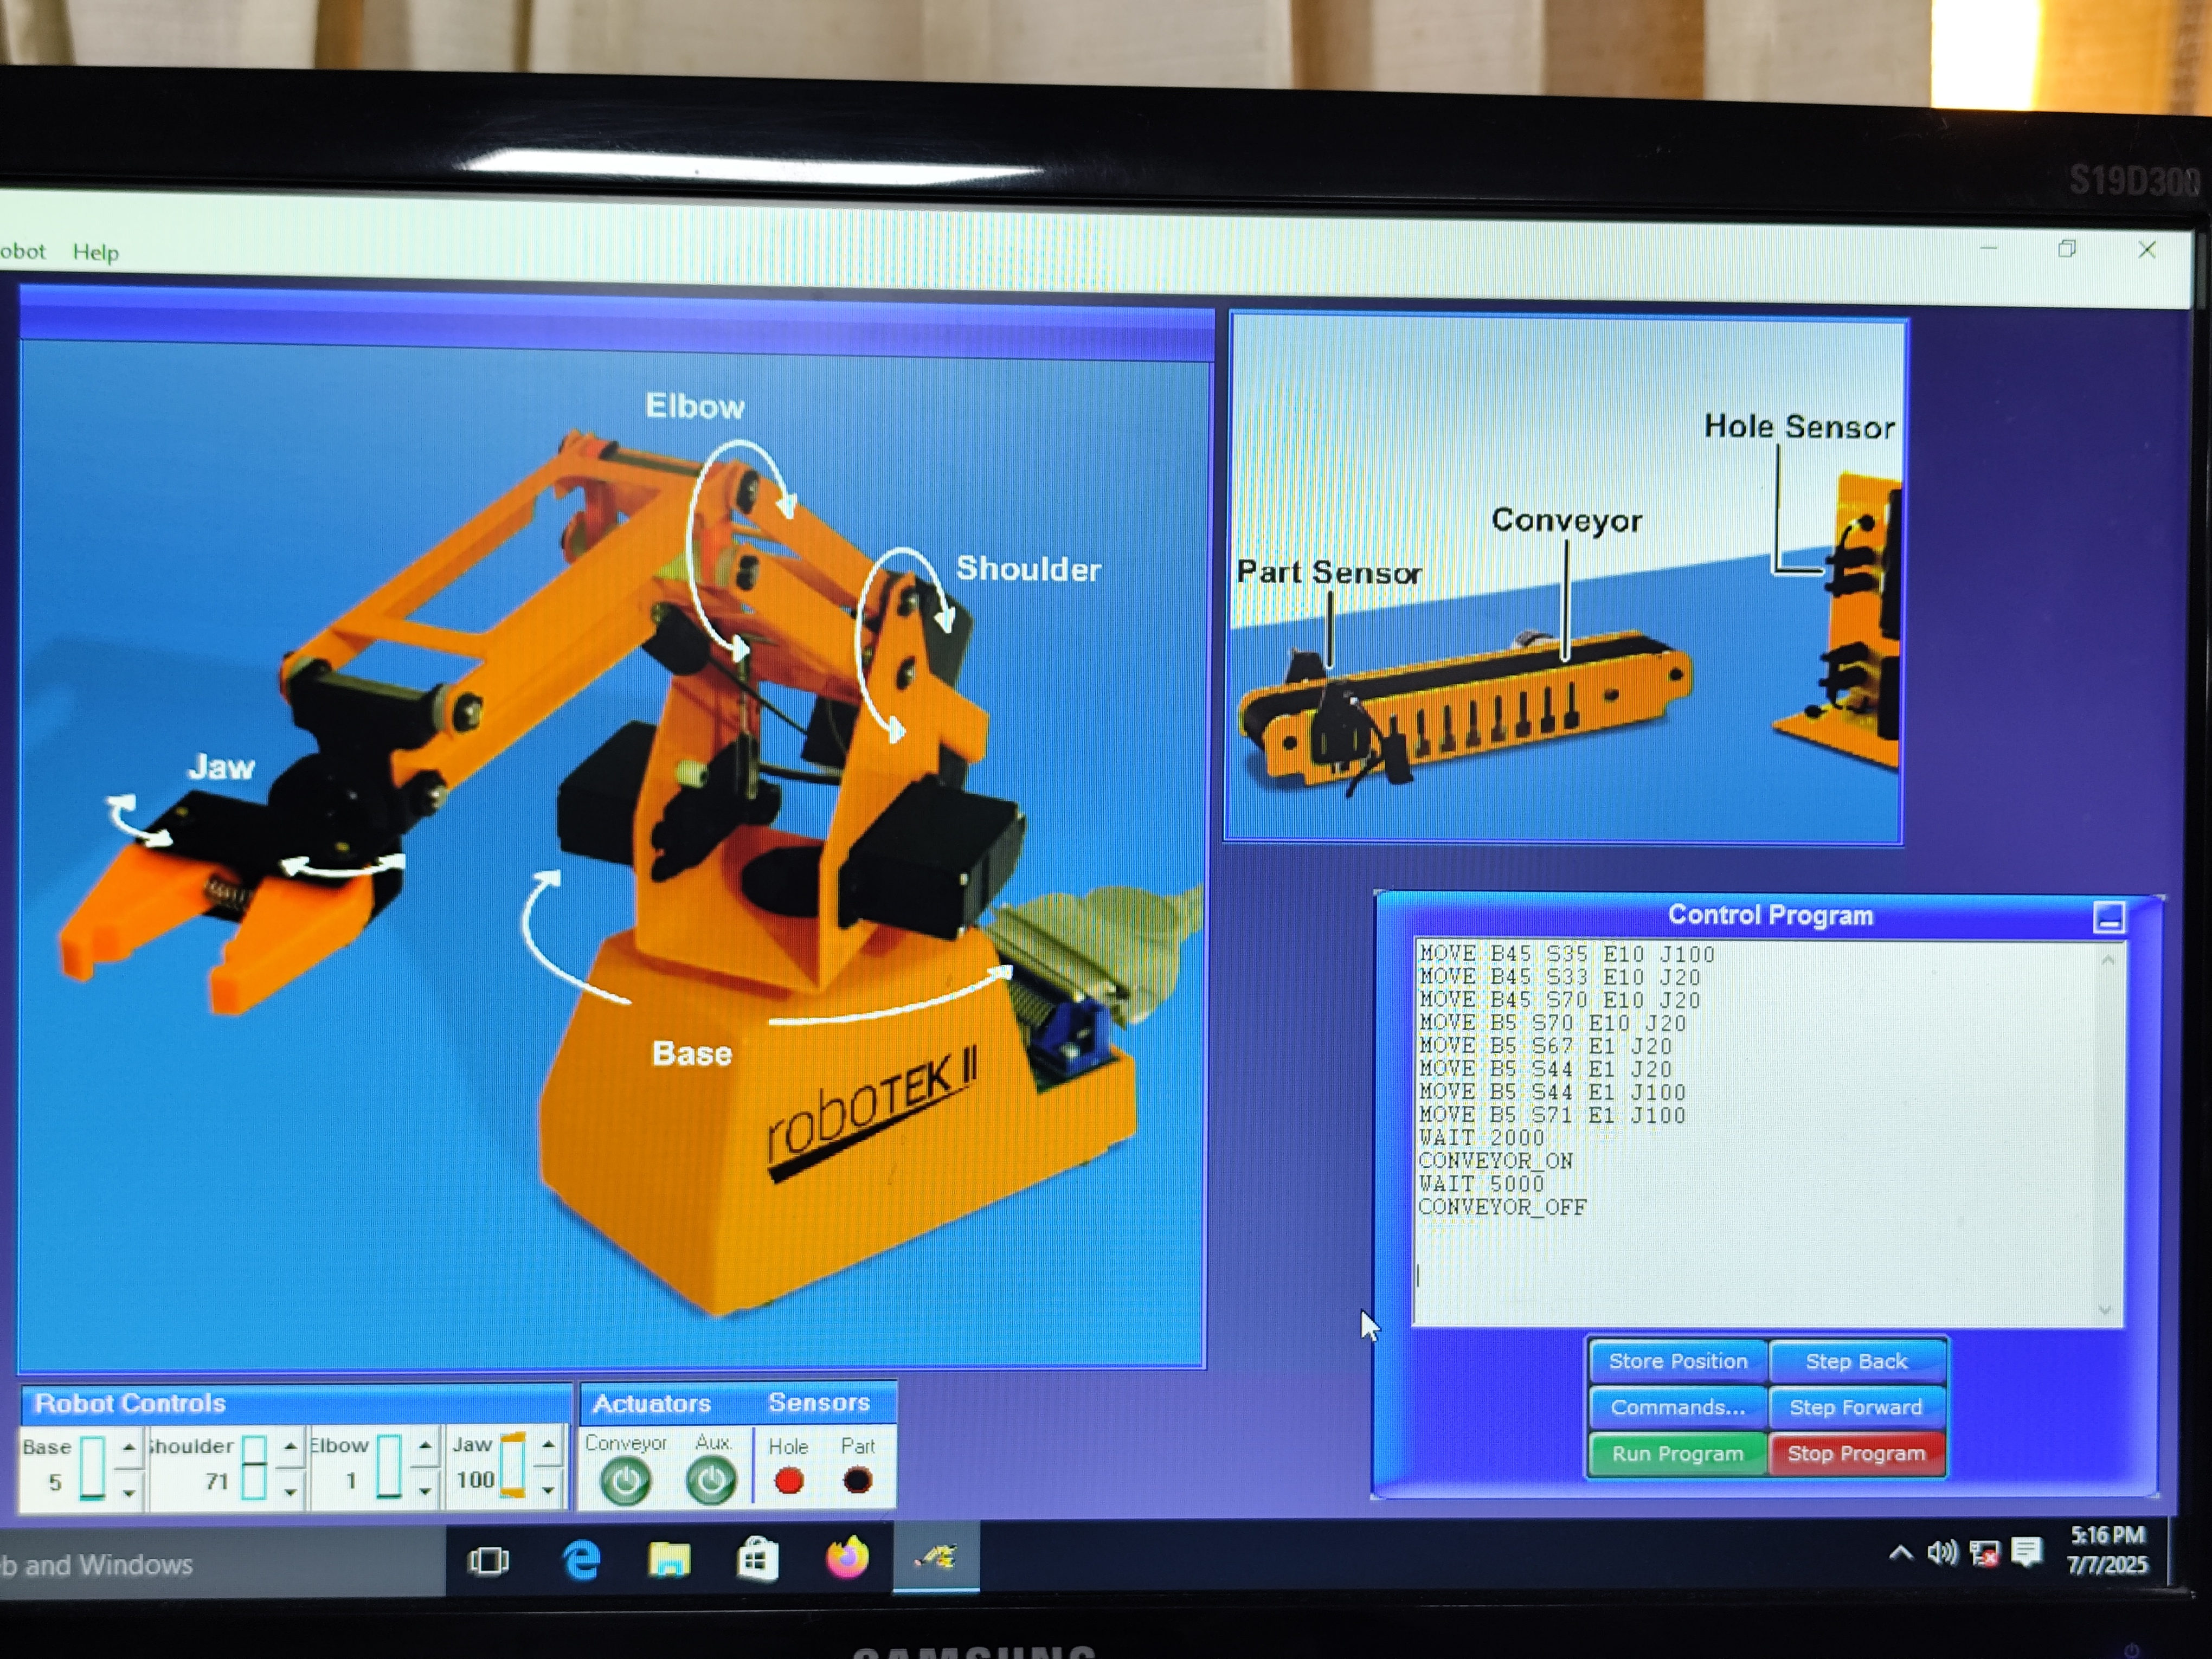
\includegraphics[width=0.8\textwidth]{2.jpg}
    \caption{Robot Control Software Interface}
    % \label{fig:Display Interface of Oscilloscope}
\end{figure}

Key software functionalities include:
\begin{enumerate}
    \item \textbf{End-Effector Control}: Accurate manipulation for pick, hold, and release tasks.
    \item \textbf{Path Planning}: Optimized movement paths for efficient positioning.
    \item \textbf{Trajectory Control}: Smooth and precise motion control.
    \item \textbf{Kinematics}: Relates joint movements to end-effector position.
    \item \textbf{Sensor Integration}: Real-time data collection for adaptive operation.
    \item \textbf{Real-Time Monitoring}: Immediate feedback for safe operation.
    \item \textbf{Programming Flexibility}: Customizable programs for varied tasks.
\end{enumerate}


\section*{Working Principle}
\addcontentsline{toc}{section}{Working Principle}
The working principle of the industrial robotic trainer kit for pick-and-place operation is summarized as follows:

\begin{itemize}
    \item The object position was identified and programmed using control software.
    \item The gripper was prepared and moved to the object location.
    \item The object was grasped and transferred to the conveyor belt.
    \item The object was released onto the conveyor, which was activated to move it to the designated box.
    \item The pick-and-place cycle was completed as the object fell into the box.
\end{itemize}

\begin{figure}[H]
    \centering
    \begin{minipage}{0.48\textwidth}
        \centering
        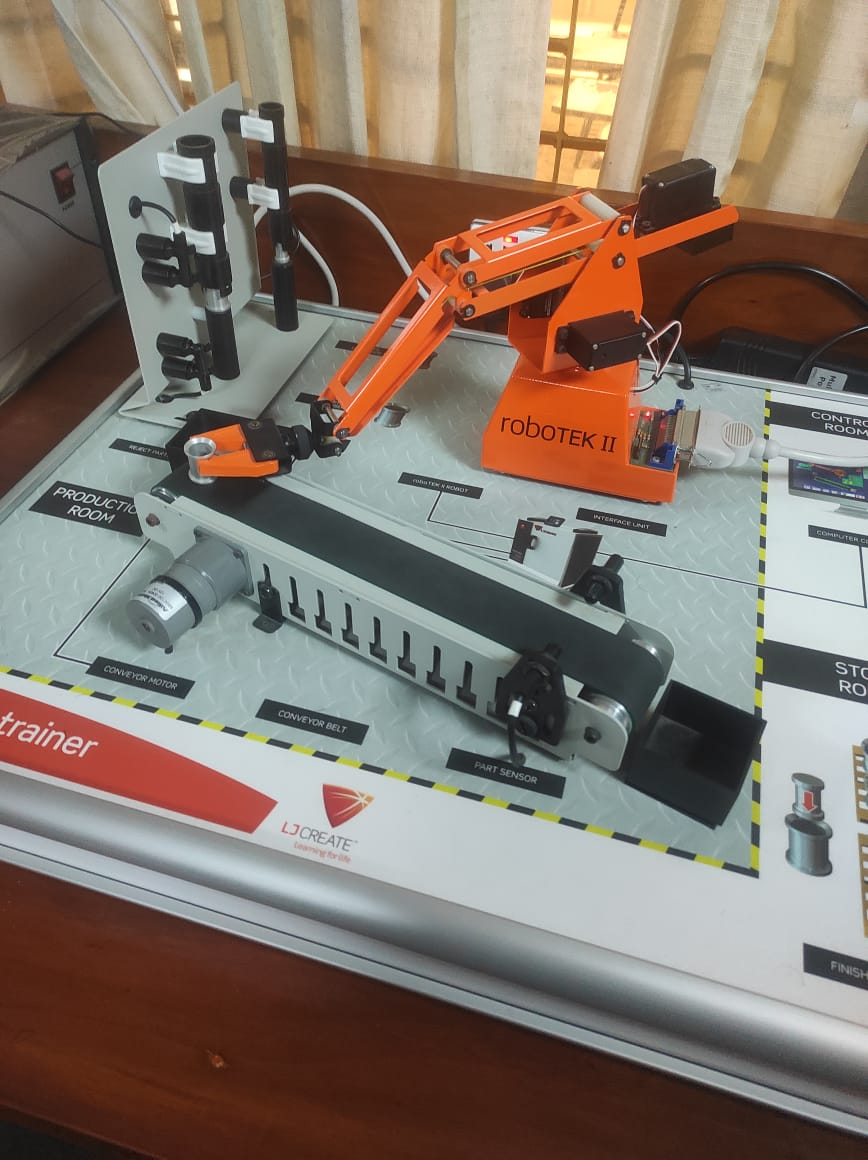
\includegraphics[width=\textwidth]{3.jpeg}
        \caption{(a) Placing the Object on the Conveyor Belt}
    \end{minipage}\hfill
    \begin{minipage}{0.48\textwidth}
        \centering
        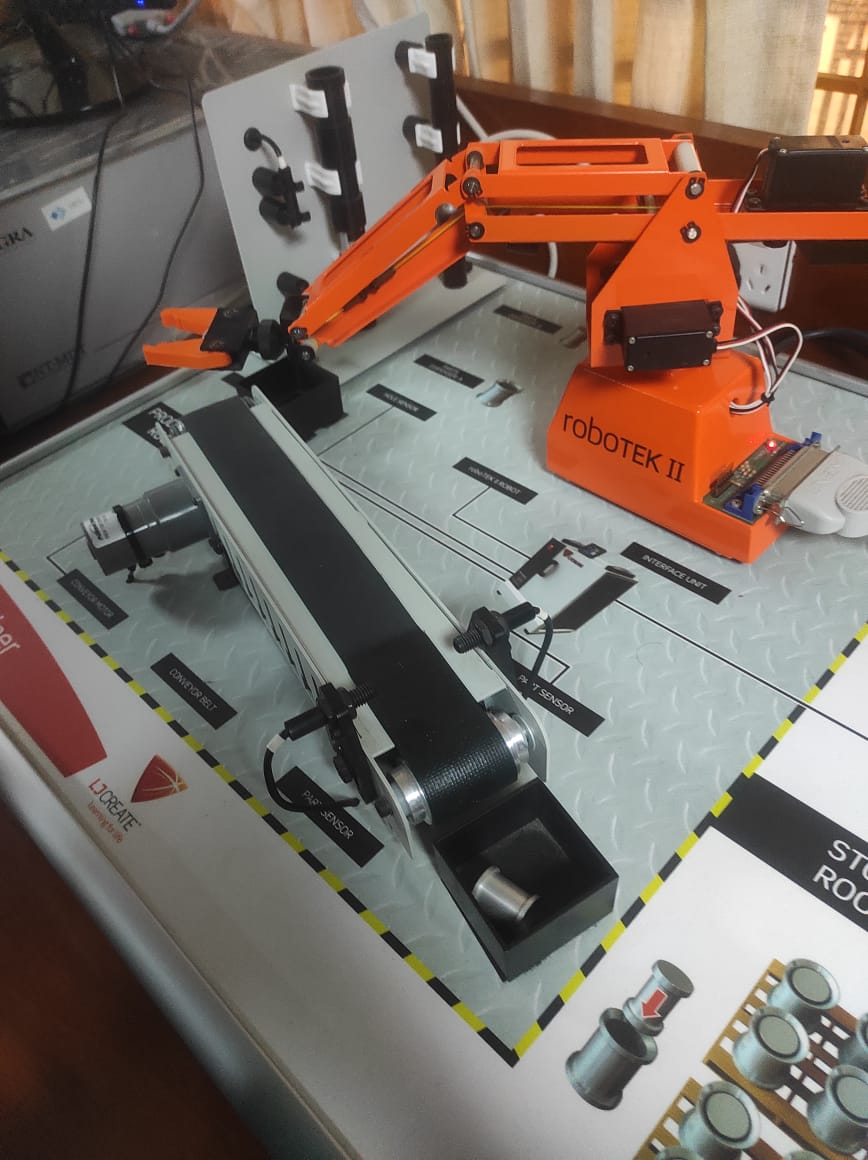
\includegraphics[width=\textwidth]{4.jpeg}
        \caption{(b) Object Falling into the Box at the end of the Conveyor Belt}
    \end{minipage}
    % \label{fig:trainer-kit}
\end{figure}

\subsection*{Code}
\addcontentsline{toc}{subsection}{Code}
\begin{minted}[fontsize=\small, bgcolor=gray!10, frame=lines]{asm}
MOVE B45 S35 E10 J100 
MOVE B45 S33 E10 J20 
MOVE B45 S70 E10 J20 
MOVE B5 S70 E10 J20 
MOVE B5 S67 E1 J20 
MOVE B5 S44 E1 J20 
MOVE B5 S44 E1 J100 
MOVE B5 S71 E1 J100 
WAIT 2000 
CONVEYOR_ON 
WAIT 5000 
CONVEYOR_OFF
\end{minted}

This procedure demonstrates the integration of robotic manipulation and automation, utilizing both software programming and hardware control to perform a typical industrial task.

\section*{Results}
\addcontentsline{toc}{section}{Results}
During the experiment, the industrial robotic trainer kit was successfully used to perform pick-and-place operations. The manipulator was programmed to identify the position of objects, grasp them using the end-effector, and transfer them onto the conveyor belt. The conveyor then transported the objects to the designated box.

Key observations:
\begin{itemize}
    \item The robot control software allowed precise control of joint movements and end-effector actions.
    \item Sensor integration enabled accurate detection of object positions and conveyor status.
    \item The pick-and-place cycle was completed reliably, with minimal errors in object handling.
    \item Real-time monitoring provided immediate feedback, ensuring safe and efficient operation.
\end{itemize}

Photographs and screenshots of the setup and software interface were taken to document the process. The experiment demonstrated the effectiveness of the trainer kit in simulating industrial automation tasks.

\subsection*{Discussion}
\addcontentsline{toc}{subsection}{Discussion}
The capabilities of the industrial robotic trainer kit in simulating automation tasks were demonstrated through successful pick-and-place operations. Precise and repeatable movements were achieved, with sensor integration enhancing accuracy and reliability. Real-time monitoring and control software features were utilized to ensure safe operation.

Some limitations were encountered, such as occasional misalignment of the gripper, which required manual adjustment. The speed and smoothness of manipulator movements were found adequate for educational use but may need improvement for industrial applications. Valuable experience in programming and troubleshooting robotic systems was gained, reinforcing theoretical concepts in automation.

\subsection*{Conclusion}
\addcontentsline{toc}{subsection}{Conclusion}
In conclusion, the industrial robotic trainer kit provided a practical platform for understanding the fundamentals of robotic manipulation and automation. Through hands-on experimentation, the pick-and-place operation was successfully implemented, demonstrating the integration of hardware and software in industrial robotics. The experience reinforced key concepts such as kinematics, sensor integration, and real-time control, highlighting the importance of precise programming and system monitoring. Overall, the experiment contributed to a deeper understanding of industrial automation and prepared participants for future applications in robotics and manufacturing.


\bibliographystyle{IEEEtran}
\renewcommand{\bibname}{References}
\addcontentsline{toc}{section}{References}
\bibliography{ref}

\end{document}
